\documentclass{article}
\usepackage[english]{babel}
\usepackage[T1]{fontenc}
\usepackage{amsmath}
\usepackage{gfsdidot}

% Graphics
\usepackage{graphicx}
\usepackage{xcolor}
\usepackage{geometry}
\geometry{
 a4paper,
 total={170mm,257mm},
 left=20mm,
 top=20mm,
}
\usepackage{caption}
\usepackage{subcaption}

% Math
\usepackage{algorithm}
\usepackage[noend]{algpseudocode}

% Links
\usepackage{hyperref}
\usepackage{url}

% Citing
\usepackage{apacite} 
\bibliographystyle{apacite}
\newcommand\shortcites[1]{\shortciteauthor{#1}'s\ \citeyear{#1}}



\title{\vspace{-0.8cm}Self-organisation of vowel systems in scale-free networks}
\author{Wolf De Wulf}
\date{}

\begin{document}
\maketitle

\begin{abstract}
    Simulations in agent-based systems that model populations of communicating agents have been used to show that due
    to
    interactions between these agents and self-organisation, realistic vowel systems emerge. Various independent
    studies
    have reported this phenomenon under various parameter configurations. The models used in these studies range from
    modelling only what is necessary to demonstrate emergence to modelling complex real life factors to investigate the
    impact on the emerged vowel repertoires. A common factor in a lot of these studies is the unrealistic assumption
    that
    every agent regularly communicates with every other agent. This article presents the analysis of a reimplementation
    of
    one of the first agent-based models that was created to analyse emergence in vowel systems. The model is extended
    to
    run simulations in scale-free networks. While scale-free networks are known to be rare in real life society, the
    simulations that were ran have allowed for gaining insights into the biases of the original system and into how it
    could be made to model society more accurately.
\end{abstract}

\section{Introduction}
It has been known for some time now that self-organisation through repeated interactions between people explains more
about the evolution of the sound systems of humans than innate predispositions do.
\shortciteA{liljencrantsNumericalSimulationVowel1972} showed that realistic vowel systems emerge when a measure of
energy, based on thermodynamic statistics, is optimised in an acoustic space of vowels. After
that,~\shortciteA{deboerSelforganizationVowelSystems2000} was the first to model a small population of agents that can
communicate with each other through a number of steps that are together deemed the `imitation game'. The agents
in~\shortcites{deboerSelforganizationVowelSystems2000} model had no innate predispositions and were still able to
converge to a global and realistic vowel system. Thereby showing that innate predispositions are not needed to explain
the evolution of vowel systems. However,~\shortcites{deboerSelforganizationVowelSystems2000} model contained a number
of ad hoc methods that could have been left out without influencing the results. Successing models such as those
by~\shortciteA{oudeyerSelfOrganizationSpeechSounds2005} and~\shortciteA{deboerMultiAgentSimulationsEvolution2010} did
so successfully while also investigating other questions such as whether or not agents should explicitly be able to
communicate or not and whether combinatorial structure emerges when instead of single vowels, sequences of vowels are
modelled. A common factor in the older models and even in most of the newer models is the assumption that every agent
regularly communicates with every other agent. In reality such fully connected networks are only found in very small
communities or in families. Therefore, these models might not capture dynamics that are present in large real life
populations. To address this, the model that is presented in this article
reimplements~\shortcites{deboerSelforganizationVowelSystems2000} model to run its simulations in a scale-free network.

Scale-free networks are networks whose degree distribution follows a power law. Such networks consist of two types of
nodes: nodes with a high degree called `hubs' and nodes with a small degree. While many real life networks were thought
to be scale-free, recent studies involving new rigorous statistical analysis techniques have showed that this is not
the case~\shortcite{clausetPowerLawDistributionsEmpirical2009,broidoScalefreeNetworksAre2019}. Examples of networks
that are thought to be scale-free are financial
networks~\shortcite{demasiFitnessModelItalian2006,soramakiTopologyInterbankPayment2007}, computer networks such as the
internet~\shortcite{faloutsosPowerlawRelationshipsInternet1999} and some social networks such as the co-authorship of
papers~\shortcite{newmanStructureScientificCollaboration2001}.
In the context of modelling a population, the idea of social networks following a scale-free structure is interesting.
Even though a network of, for example, co-authorship in mathematical papers is not one in which phonology plays an
important role, investigating what happens when an agent-based model that is designed to model a population of
communicating agents is adapted to run its simulations in such a network, should prove to be insightful. This is
exactly the case for the~\shortcites{deboerSelforganizationVowelSystems2000} model. The reimplementation of this model
that is presented in this article shows that the ad hoc methods
that~\shortciteA{deboerSelforganizationVowelSystems2000} uses to model agents introduces a model-specific bias.
Insights into how the model can be adjusted to generalise to more realistic networks are gained through a number of
experiments.

In what follows, Section~\ref{sec:SF} gives an in depth discussion on scale-free networks, the methods that can be used
to generate them and their . Subsequently, Section~\ref{sec:methods} repeats the architecture
of~\shortcites{deboerSelforganizationVowelSystems2000} model and the adjustments that are made for it to run its
simulations in scale-free networks. Afterwards, Section~\ref{sec:exp} establishes a number of experiments of which
Section~\ref{sec:discus} discusses the results. Section~\ref{sec:conclusion} concludes the article with a number of
conclusions and possible future work.

\section{Scale-free networks\label{sec:SF}}
Scale-free networks are networks whose degree distribution asymptotically follows a power law. In a pure scale-free
network the probability of a node to have $k$ edges to other nodes is defined as follows:
\begin{align}
    P(k) \sim k^{-\gamma}
\end{align}
with $\gamma$ a scaling parameter typically in the range $2 \leq \gamma \leq 3$. Evidence for scale-free structure in a
network can be found using statistical techniques. \shortciteA{broidoScalefreeNetworksAre2019} summarise the different
notions of evidence in a set of categories which are not repeated here. For the rest of this article it suffices to
know that the used scale-free networks belong to the ``strongest'' category, which is due to the method that is used to
generate them. The scale-free networks in this article are generated using the most known mechanism to do so, called
preferential attachment~\shortcite{albertStatisticalMechanicsComplex2002}. The preferential attachment mechanism to
generate a scale-free network of size $N$ is given by Algorithm~\ref{alg:PA}.

\begin{algorithm}
    \caption{Preferential attachment \protect\shortcite{albertStatisticalMechanicsComplex2002}}\label{alg:PA}
    \begin{algorithmic}[1]
        \State $net \gets fully\_connected(4);$
        \While{$net.size() < N$}
        \State $A \gets net.new\_node();$
        \State $count \gets 4;$
        \While{$count != 0$}
        \State $B \gets net.random\_node();$
        \If{$!net.connected(A,B)$}
        \State $net.connect(A,B) \textbf{ with probability } \frac{B.degree}{net.total\_degree}$
        \EndIf
        \EndWhile
        \EndWhile
    \end{algorithmic}
\end{algorithm}
\noindent
The mechanism starts by initialising the network as a fully connected network of four nodes. Subsequently, the network
is expanded by adding nodes until the network consists of $N$ nodes. Each time a node is added, the following steps are
repeated 4 times: select a random node from the network, if the random node is not connected to the new node, connect
them with probability:
\begin{align*}
    P(k_i) = \frac{k_i}{\sum_{j} k_j}
\end{align*}
where $k_i$ is the degree of the randomly selected node. Hence, preferential attachment is a probabilistic mechanism.
New nodes are allowed to connect to any other node in the network. However, if a new node can be connected to a node
with degree 2 or to a node with degree 4, the node with degree 4 is twice as likely to be chosen.

Whether or not preferential attachment can be used to accurately describe a population of humans is a topic that has
sparked a lot of debate. Intuitively, the `hubs' created by the preferential attachment mechanism seem to be realistic.
By varying the scale and the context of the community a scale-free network is supposed to model, its adequacy varies as
well. Take, for example, a university community consisting of professors and students. In such a case, a scale-free
network seems like an adequate depiction of the underlying network. On the other hand, a much smaller community of
hunter-gatherers might be more accurately modelled by a fully connected network. By analysing a variety of real life
networks,~\shortciteA{broidoScalefreeNetworksAre2019} came to the conclusion that social networks are at best `weakly'
scale-free. Nevertheless, making models such as those by~\shortciteA{deboerSelforganizationVowelSystems2000}
and~\shortciteA{oudeyerSelfOrganizationSpeechSounds2005} run their simulations in large and complex social networks
would result in incorrect representations of reality. When sound systems started emerging for the first time, social
networks were surely much smaller and simpler than those analysed by~\shortciteA{broidoScalefreeNetworksAre2019}.
Similarly to how language is said to be the result of the co-evolution of biological and cultural
inheritance~\shortcite{deboerBiologyCultureCoevolutionFinite2018}, the evolution of language and the structure of
society are two concurrent evolutionary processes that influence each other. Therefore, modelling an evolving sound
system in a fixed network structure is not realistic. A more realistic introduction of network structure into models
that investigate the emergence of sound systems would require network structure to evolve as well. This does not mean
that looking at what happens when a particular fixed network structure is added to a model that investigates the
emergence of vowel systems is entirely useless. While the speeds at which language and societal structure evolve are
likely to be much more comparable than those of biological and cultural inheritance, fixing network structure in a
model can still provide insights into one direction of the co-evolution, namely, the influence of network structure on
the evolution of language.

\begin{figure}[t]
    \centering
    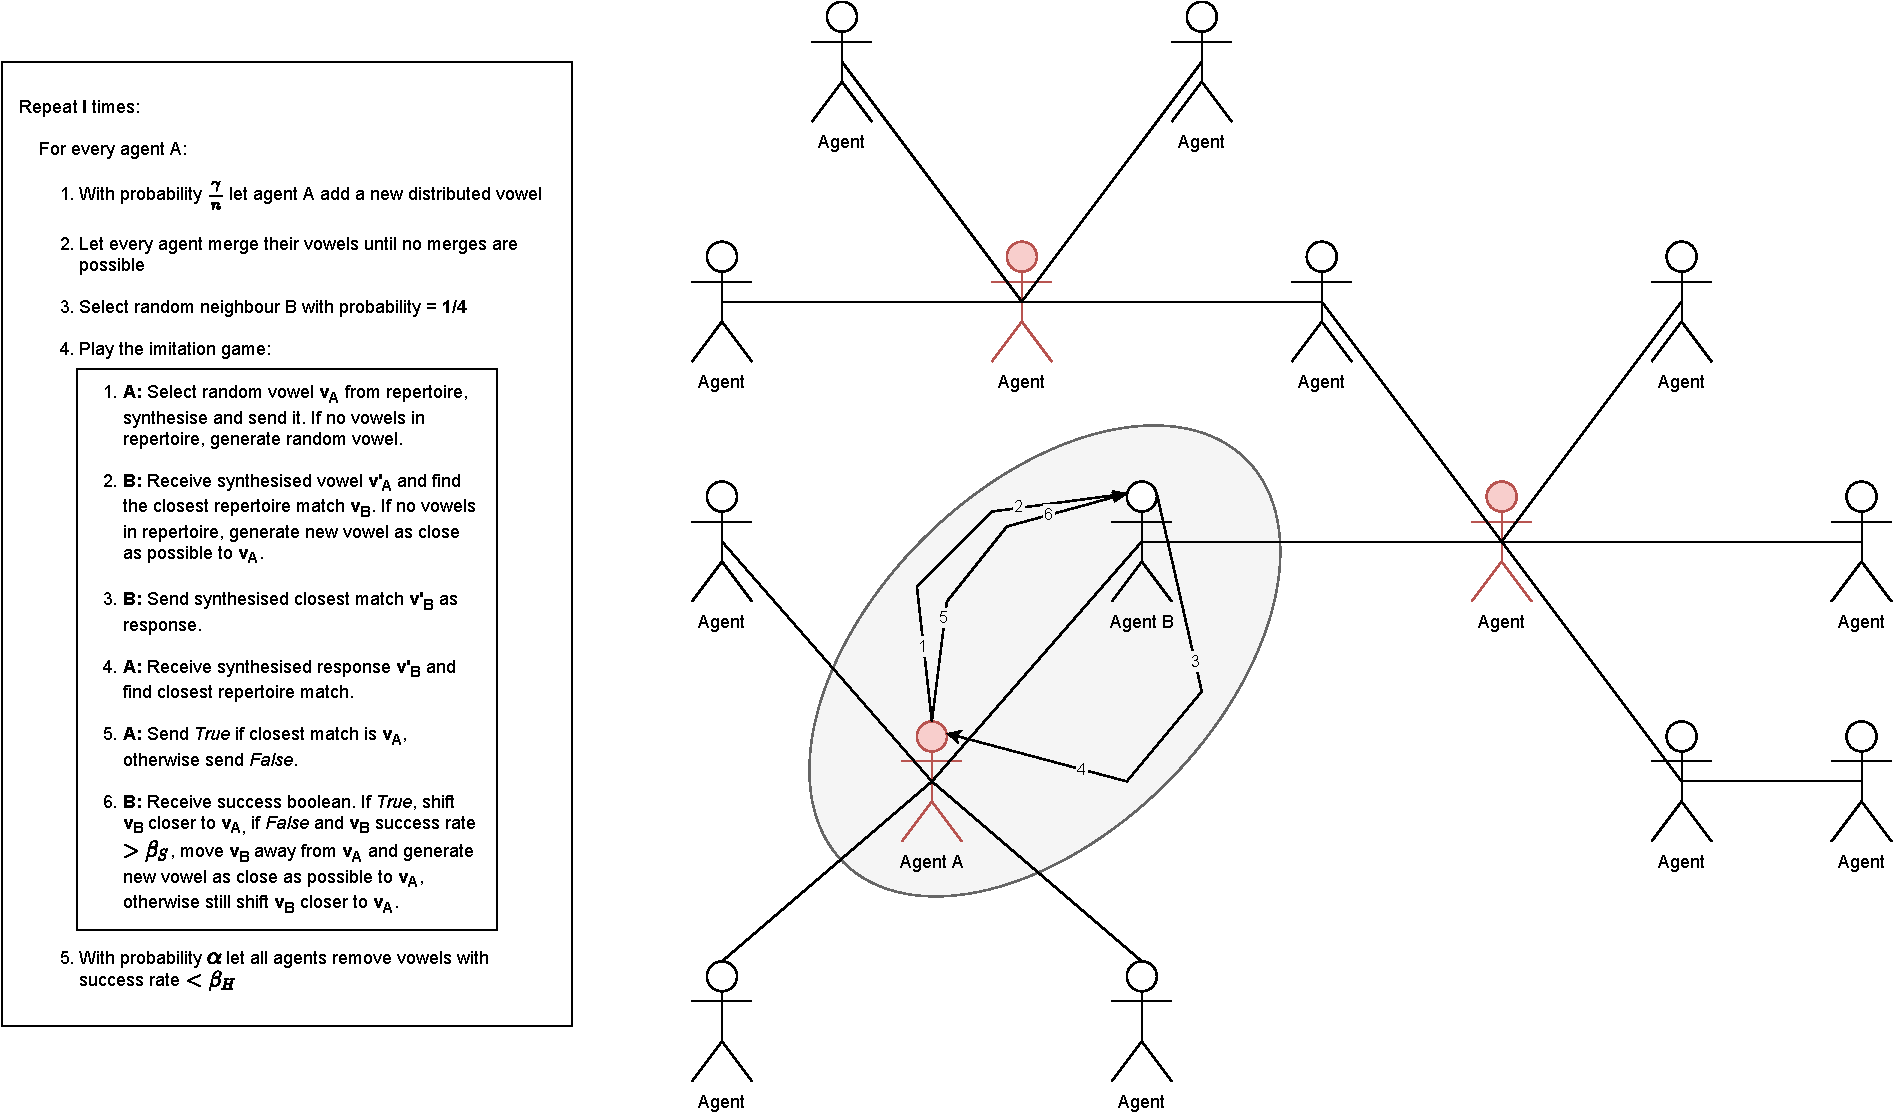
\includegraphics[width=\textwidth]{figures/simulation_diagram.pdf}
    \caption{Graphical representation of the steps that are executed during a simulation.}
    \label{fig:model}
\end{figure}

\section{Methodology\label{sec:methods}}
Aside from two changes, the model\footnote{The source code of the model can be found on GitHub:
    \url{https://github.com/wulfdewolf/ProjectEoS}} that is presented here is exactly the same as that
of~\shortciteA{deboerSelforganizationVowelSystems2000}. Originally, the model was implemented in C++ and while this did
not change, the model was reimplemented for compatibility reasons. The two aspects that were adapted in  the first
model are the following: the network architecture in which the simulations run and the bark-to-hertz and hertz-to-bark
conversions.

Figure~\ref{fig:model} gives a graphical representation of the steps that are executed during a simulation. Each
iteration starts by selecting a random agent $A$ from the complete population. Agent $A$ is the \textit{sender} of the
iteration. With probability $\frac{1}{100}$, agent $A$ is allowed to add a new distributed vowel to their repertoire.
The distribution of vowels is implemented just as it was by~\shortciteA{deboerSelforganizationVowelSystems2000}: by
maximising the distance to all other vowels. Subsequently, every agent merges vowels that are too alike until no merges
are possible. The merging threshold is $0.17$ in articulatory space and $\frac{log(1+noise)}{0.1719} -
    \frac{log(1-noise}{0.1719}$, defined by~\shortciteA{deboerSelforganizationVowelSystems2000} to be the maximum
distance
a vowel can be shifted by ambient noise, in acoustic space.
After merging, a random neighbour $B$ of agent $A$ is chosen to be the receiver of the iteration.
Originally,~\shortciteA{deboerSelforganizationVowelSystems2000} chose the receiver agent as a random agent from the
complete population, thereby modelling a fully connected network. Once a sender and a receiver have been chosen, an
imitation game is played. Agent $A$ chooses a random vowel $v_A$ from their repertoire, synthesises it, and sends it to
agent $B$ as an utterance $v'_A$, thereby adding a $10\%$ noise shift. If agent $A$'s repertoire was empty, it is
initialised with a completely random vowel. Agent $B$ hears the synthesised vowel $v'_A$ and finds the most resembling
vowel $v_B$ in their repertoire, synthesises it, and sends it to agent $A$ as an utterance $v'_B$, once more, adding a
$10\%$ noise shift. Agent $A$ hears agent $B$'s response and finds the most resembling vowel in their repertoire. If
this vowel is the original $v_A$ then the imitation game was successful and agent $A$ sends \textit{True} to agent $B$,
otherwise the imitation game failed and agent $A$ sends \textit{False} to agent $B$. Lastly, agent $B$ receives the
success boolean and does the following. If it is \textit{True}, agent $B$ moves $v_B$ closer to $v_A$, since by
uttering $v_B$ agent $A$ was able to understand agent $B$. If it is \textit{False} and the success rate of $v_B$ is $>
    0.5$ then agent $B$ moves $v_B$ away from $v_A$ and adds a new vowel as close as possible to $v_A$. The reasoning
behind this is that $v_B$ is not a bad vowel because it is successful half of the times it is used. It is rather that
agent $A$ probably has another vowel that is closer to $v_B$ than $v_A$ is. Therefore, agent $B$ should learn this
vowel. If the received boolean is \textit{False} and the success rate of $v_B$ is $\leq 0.5$, then agent $B$ still
moves $v_B$ closer to $v_A$, however, this does not add to the success rate of $v_B$. Finally, after the imitation game
and with a probability of $\frac{1}{10}$, every agent is allowed to remove the bad vowels from their repertoires.
Vowels that have been used at least 5 times and have a success rate $< 70\%$ are removed. As mentioned, the network
that decides an agent's neighbours is generated using Algorithm~\ref{alg:PA}. Synthesising, shifting vowels and
distance measures are all implemented as they were by~\shortciteA{deboerSelforganizationVowelSystems2000}.

The bark-to-hertz and hertz-to-bark conversions that were implemented
by~\shortciteA{deboerSelforganizationVowelSystems2000} are interpolations based on data from other papers. The second
adaptation to~\shortcites{deboerSelforganizationVowelSystems2000} model is the implementation of the conversions that
are implemented in
MATLAB\footnote{\url{https://nl.mathworks.com/help/audio/ref/bark2hz.html}}\footnote{\url{https://nl.mathworks.com/help
        /audio/ref/hz2bark.html}}, which are based on the work
of~\shortciteA{traunmullerAnalyticalExpressionsTonotopic1990}:
\begin{align}
    bark & = \begin{cases}
        \frac{bark - 0.3}{0.85}   & \text{ if } bark < 2    \\
        \frac{bark + 4.422}{1.22} & \text{ if } bark > 20.1 \\
        bark                      & \text{ otherwise}
    \end{cases}
\end{align}
and:
\begin{align}
    bark & = \frac{26.81 * hertz}{1960 + hertz} - 0.53 \\
    bark & = \begin{cases}
        bark + 0.15 * (2- bark)     & \text{ if } bark < 2    \\
        bark + 0.22 * (bark - 20.1) & \text{ if } bark > 20.1 \\
        bark                        & \text{ otherwise}
    \end{cases}
\end{align}
While different conversions will most likely not change much in the results, for comparability it is better to use some
standardized implementation.

\section{Experiments\label{sec:exp}}
Two types of experiments are established. Firstly, the experiment and evaluation from Section 4.1
from~\shortcite{deboerSelforganizationVowelSystems2000} is reproduced. This serves to demonstrate that the
reimplementation of the model is correct. Both are also done for an instance of the model that runs its simulations in
a scale-free network. By comparing the results of the two, insights can be gained regarding the research question that
is addressed here. Additionally, for both models, a second experiment is conducted to investigate the influence of the
population size on the results. Due to the difference in network structure of the two models it is reasonable to expect
different results for this experiment.

The first experiment consists of investigating the emergence of a vowel system in a population of 20 agents under 10\%
acoustic noise.
\shortciteA{deboerSelforganizationVowelSystems2000} analyses the combined acoustic repertoires of all agents after 20,
500, 2000, and 10000 imitation games. The robustness of the emerged results is evaluated by repeating the simulations
1000 times for 5000 imitation games and plotting the success, size, and energy distributions. Both of these evaluations
are repeated here. While the remaining other experiments from \shortcite{deboerSelforganizationVowelSystems2000} could
also be repeated, since the model here is a reimplementation, the mentioned experiments should be enough to show that
the reimplementation was done correctly. Running the other experiments for an instance of the model that runs its
simulations in a scale-free network could also be interesting but it is not done in this article.

To allow for correct comparisons in the experiments where population sizes are varied,
~\shortciteA{deboerSelforganizationVowelSystems2000} implements two changes in the model. Firstly, the number of games
is kept per agent and not globally, hence, smaller populations play a smaller number of imitation games. Secondly, the
probability of adding new distributed vowels must be made dependent on the number of games per agent instead of on the
global number of played games. Therefore, the probability of adding new distributed vowels is set to $\frac{0.2}{N}$,
with $N$ the number of agents in the population. \shortciteA{deboerSelforganizationVowelSystems2000} chose 0.2 as
denominator such that for a population of 20 agents the insertion probability is $1\%$. Both of these changes are
implemented here as well.

\section{Discussion\label{sec:discus}}

\section{Conclusions\label{sec:conclusion}}

\bibliography{refs}
\end{document}